\documentclass[lang=cn,math=cm,chinesefont=nofont,11pt,scheme=chinese,onecol]{elegantbook}
\setCJKmainfont[BoldFont={FZHei-B01},ItalicFont={FZKai-Z03}]{FZShuSong-Z01}
\setCJKsansfont{FZHei-B01}
\setCJKfamilyfont{zhsong}{FZShuSong-Z01}
\setCJKfamilyfont{zhhei}{FZHei-B01}
\setCJKfamilyfont{zhkai}{FZKai-Z03}
\setCJKfamilyfont{zhfs}{FZFangSong-Z02}
\setCJKfamilyfont{zhli}{FZLiShu-S01}

\newcommand*{\songti}{\CJKfamily{zhsong}} % 宋体
\newcommand*{\heiti}{\CJKfamily{zhhei}} % 黑体
\newcommand*{\kaiti}{\CJKfamily{zhkai}} % 楷体
\newcommand*{\fangsong}{\CJKfamily{zhfs}} % 仿宋
\newcommand*{\lishu}{\CJKfamily{zhli}}    % 隶书
\linespread{1.3}

\usepackage{graphicx}

\title{数学之桥:从初等数学到微积分}
\subtitle{Powered by \LaTeX.}

\author{Siliconet}
\date{始于2023年}
\version{1.0}
\bioinfo{模板}{ElegantBook}

\extrainfo{你站在桥上看风景,看风景人在楼上看你。明月装饰了你的窗子,你装饰了别人的梦。}

\setcounter{tocdepth}{3}

\cover{cover.jpg}

% 本文档命令
\usepackage{array}
\newcommand{\ccr}[1]{\makecell{{\color{#1}\rule{1cm}{1cm}}}}

% 修改标题页的橙色带
\definecolor{customcolor}{RGB}{255,255,255}
\colorlet{coverlinecolor}{customcolor}
\usepackage{cprotect}

\addbibresource[location=local]{reference.bib} % 参考文献,不要删除

\setcounter{tocdepth}{1}
%设置目录显示深度

\begin{document}

\maketitle
\frontmatter

\tableofcontents

\mainmatter

\chapter{集合论初步}

本项目采用ElegantBook作为模板,模板地址:

GitHub:\href{https://github.com/ElegantLaTeX/ElegantBook}{https://github.com/ElegantLaTeX/ElegantBook}

CTAN:\href{https://ctan.org/pkg/elegantbook}{https://ctan.org/pkg/elegantbook}

本书的GitHub开源地址:

\href{https://github.com/Siliconet/Math-Bridge}{https://github.com/Siliconet/Math-Bridge}

\section{集合的概念与表示}
集合论是学习数学的基础。基础到什么地步呢?集合论在几乎所有其他数学分支领域中都是基础内容。一方面,它作为一种表示工具存在。集合可以用来表示各种东西,比如说奇数、偶数、质数、合数。另一方面,集合是逻辑推理的基础,这意味着要继续学习接下来的内容,先学集合是必不可少的。(没错下一章就是简易逻辑,虽然集合论远不止于此)

那为什么不从小学开始学呢?普通小学生一开始学不懂嘛。

\subsection{集合的概念}

你没看错,这一节是集合的概念,而不是集合的定义。为什么呢?因为集合根本就没有定义!集合是一个数学上的基本概念,或者说,是一个\textbf{本原概念}。但是我们可以给出一个对于集合这个概念的描述:


\textbf{集合}(简称\textbf{集})是一些具有某种特定性质的对象组成的总体。

怎么理解这个特定性质呢?比如说,身高高于165cm算不算一个特定性质?显然算嘛。所以我们可以这么说:“我的班上身高高于165cm的同学”能构成一个集合。

满足某个特定的不等式算不算特定性质?算。于是解集(你在初中已经见过)这个概念诞生了,就是解的集合。

我们研究的很多东西都可以构成集合。构成集合的对象可以是各种事物,可以是物,也可以是人,可以是数,也可以是图形,甚至可以是集合(没错就是套娃)……构成集合的对象称为这个集合的\textbf{元素}。

比方说,以2023年《财富》世界500强排行榜当中的前5名作为一个集合,那么这个集合的元素是:沃尔玛、沙特阿美公司、国家电网有限公司、亚马逊、中国石油天然气集团有限公司。

按照集合中含有的元素的个数,我们把集合分成两类:\textbf{有限集}(含有有限个元素的集合)和\textbf{无限集}(含有无限个元素的集合)。

这里还要提到两种特别的集合:

\textbf{空集}(记作$\varnothing$)是不含任何元素的集合;

\textbf{单元素集}是只含一个元素的集合。

我们通常用英文大写字母$A$,$B$,$C$,$\cdots$表示集合,用小写英文字母$a$,$b$,$c$,$\cdots$表示集合的元素。

如果$a$是集合$A$的元素,我们就记作$a\in A$,读作“$a$属于$A$”,与此相反的情况是,如果$a$不是集合$A$的元素,我们就记作$a\notin A$,读作“$a$不属于$A$”。

那么问题来了,$\varnothing \in \{\varnothing\}$是不是正确的?是。因为$\varnothing$是$\{\varnothing\}$当中的一个元素,二者并不相同。

\subsection{集合的特性}
集合有以下三个特性:\textbf{确定性、互异性、无序性}。

所谓确定性,指的是集合中的每一个元素都是确定的。因此,“我的班上身高比较高的同学”不能构成一个集合,因为身高的高矮之分并没有明确的标准,身高180cm算不算高?身高160cm算不算高?没有一个明确的标准是无法确定身高到底算不算“比较高”的。

所谓互异性,指的是集合中的元素都互不相同,我们只研究由不同元素构成的集合,这是为了研究的方便。

所谓无序性,指的是集合中的元素没有确定的顺序。

\subsection{常用的数集}
现在来看几个比较常用的数集:

1.所有非负整数构成的集合称为\textbf{自然数集},记作$\mathbb{N}$。友情提示,$0\in \mathbb{N}$。

2.所有正整数构成的集合称为\textbf{正整数集},记作$\mathbb{N}_+$或者$\mathbb{N}^*$。

3.所有整数构成的集合称为\textbf{整数集},记作$\mathbb{Z}$。

4.所有有理数构成的集合称为\textbf{有理数集},记作$\mathbb{Q}$。

5.所有实数构成的集合称为\textbf{实数集},记作$\mathbb{R}$。

还有一些比较特别(用得比较少)的数集,如正有理数集$\mathbb{Q}^+$,负实数集$\mathbb{R}^-$,正实数集$\mathbb{R}^+$。

此外,由点组成的集合称为\textbf{点集}。

\subsection{集合的表示}
集合有两种主要的的表示方法:\textbf{列举法}和\textbf{描述法}。

把集合里的元素全部列出来,写在花括号内,并且元素之间用逗号分隔,这种表示集合的方法称为\textbf{列举法}。

举三个例子:

\begin{example}
  12的所有因数组成的集合可以表示为$\{-12,-6,-4,-3,-2,-1,1,2,3,4,6,12\}$.
\end{example}
\begin{example}
  唐宋八大家的姓名组成的集合可以表示为$\{\text{韩愈,柳宗元,欧阳修,苏洵,苏辙,苏轼,王安石,曾巩}\}$。
\end{example}
以及圆的全新定义:
\begin{definition}[圆]
  圆是平面内与一个定点距离为定长的点的集合。
\end{definition}
这里我们只是用集合把初中学过的圆的定义重新描述了一遍。

如果一个集合的元素很多,我们可以列举几个元素表示元素的规律,其余的用省略号代替。

\begin{example}
  自然数集可以这么表示:$\{0,1,2,\cdots,n,\cdots\}$。
\end{example}

对于元素个数有限的集合,我们要把最后一个元素给写出来。
\begin{example}
  小于或等于50的自然数组成的集合可以这么表示:$\{0,1,2,\cdots,50\}$。
\end{example}


列举法当然是不能解决全部集合的表示问题的,比方说,不等式$2x\geq 0$的解集怎么用列举法表示?这时候我们就需要\textbf{描述法}了。

先举个例子。以上面这个不等式为例,满足$x\geq 0$的实数都是这个不等式解集的元素,而不满足$x\geq 0$的实数都不是。所以我们可以这么表示该解集:
$$\{x\mid x\geq0\}$$

\begin{definition}[特征性质]
如果属于集合$a$的任意一个元素$x$都具有性质$p(x)$,而不属于集合$A$的元素都不具有这个性质,则称性质$p(x)$为集合$A$的一个\underline{特征性质}。一个集合可以有多个特征性质。
\end{definition}
比方说,上面的$x\geq 0$就是上面的不等式解集的特征性质。

于是我们就可以用特征性质来表示集合:$$\{x\mid p(x)\}$$

这就是\textbf{描述法},全称是\textbf{特征性质描述法}。

\begin{example}
  所有4的倍数组成的集合为$\{x\mid x=4n,n\in\mathbb{Z}\}$。当然写成$\{\text{4的倍数}\}$也没问题。
\end{example}

\begin{example}
  不等式$2x-7\geq 0$的解集可表示为$\{x\mid x\geq\frac{7}{2}\}$,也可以直接表示成$\{x\mid 2x-7\geq 0\}$。这里我们推荐前者,因为是化简过的。
\end{example}

\begin{example}
  平面直角坐标系内第一象限的所有点组成的集合为$\{(x,y)\mid x>0,y>0\}$。把逗号换为“且”也是可以的。
\end{example}

\begin{example}
  所有的正奇数组成的集合为$\{x\mid x=2n+1,n\in\mathbb{N}\}$,也可以写成$\{x\in\mathbb{N}\mid x=2n+1,n\in\mathbb{Z}\}$,二者是一样的。
\end{example}

\begin{remark}
  对于一个集合$\{x\mid p(x)\}$,它当中所有属于另一个集合$\boldmath{I}$(我们默认研究实数范围内的数,所以$\boldmath{I}$为$\mathbb{R}$时通常省略)的元素组成的集合,可以表示为$$\{x\in\boldmath{I}\mid p(x)\}$$
\end{remark}

\begin{example}
  \label{exp:1}
  所有的奇数组成的集合为$\{x\mid x=2n+1,n\in\mathbb{Z}\}$,也可以写成$\{x\in\mathbb{Z}\mid x=2n+1,n\in\mathbb{Z}\}$,二者是一样的。奇数集还可以表示为$\{x\mid x=2n-1,n\in\mathbb{Z}\}$,甚至是$\{x\mid x=2n-3,n\in\mathbb{Z}\}$(你可以使用列举法验证这个说法的正确性),当然我们更多地使用第1、3两种。
\end{example}

如果不会引起混淆的话,竖线及其左边的部分可以省略。如所有锐角三角形构成的集合可表示为$\{\text{锐角三角形}\}$。

\subsection{区间}
区间其实是对集合的简写。
\begin{definition}[区间]
	设$a,b\in\mathbb{R}$,且$a<b$,则\\集合$\{x\mid a\leq x\leq b\}$可简写为$[a,b]$,称为\underline{闭区间};\\集合$\{x\mid a<x<b\}$可简写为$(a,b)$,称为\underline{开区间};\\集合$\{x\mid a\leq x<b\}$可简写为$[a,b)$,称为\underline{左闭右开区间};集合$\{x\mid a< x\leq b\}$可简写为$(a,b]$,称为\underline{左开右闭区间},合称\underline{半开半闭区间}。
\end{definition}

\begin{example}
  不等式$\begin{cases}3x-(x-3)\geqslant1\\\dfrac{2x+1}{3}>x-1\end{cases}$的解集为$[-1,4)$。
\end{example}

\begin{definition}[无穷区间]
    设$a\in\mathbb{R}$,则集合$\{x\mid x\geq a\}$可简写为$[a,+\infty)$,集合$\{x\mid x>a\}$可简写为$(a,+\infty)$,集合$\{x\mid x\leq a\}$可简写为$(-\infty,a]$,集合$\{x\mid x<a\}$可简写为$(-\infty,a)$。
\end{definition}

\begin{example}
  使式子$\sqrt{2x-3}$有意义的所有实数组成的集合为$[\frac{3}{2},+\infty)$。
\end{example}

\subsection{习题}

\begin{exercise}\label{exer:1}
  用符号“$\in$”或“$\notin$”填空:\\
(1)$1\_\_\_\mathbb{N}$;(2)$0\_\_\_\varnothing$;(3)$(2,7)\_\_\_\{(x,y)\mid x+2y=3\}$;(4)$-1\_\_\_\{x\mid x^{3}<2\}$;\\(5)$2024\_\_\_\{x\mid x=4n-1,n\in\mathbb{Z}\}$.
\end{exercise}

\begin{exercise}\label{exer:2}
  下列集合是有限集还是无限集?\\
  (1)$\{\text{周长等于20cm的三角形}\}$;(2)$\{\text{太阳系八大行星}\}$;(3)$\{\text{大于10的素数}\}$.
\end{exercise}

\begin{exercise}\label{exer:3}
  用列举法表示下列集合:\\
  (1)$\{x\mid x^2+2=6\}$;
  (2)绝对值小于3的所有整数组成的集合;
  (3)能整除所有自然数的数组成的集合。
\end{exercise}

\begin{exercise}\label{exer:4}
  用描述法表示下列集合:\\
  (1)平面直角坐标系第一象限内所有点的坐标;
  (2)所有矩形组成的集合;
  (3)$\{1,5,25,125,625\}$.
\end{exercise}

\begin{exercise}\label{exer:5}
  写出方程组$\left.\left\{\begin{aligned}x+y&=3\\y+z&=4\\z+x&=5\end{aligned}\right.\right.$的解集。
\end{exercise}

\begin{exercise}\label{exer:6}
  已知集合$A=\{x-2,x+5,12\}$,且$-3\in A$,求$x$的值。
\end{exercise}

\begin{exercise}\label{exer:7}
  设$P$表示平面$a$内的动点,$A,B,O$分别是平面$\alpha$内的三个定点,属于下列集合的点构成平面$\alpha$内的什么图形?\\
  (1)$\{P||PA|=|PB|\}$;
  (2)$\{P||PO|=3\text{cm}\}$
  (3)$\{P||PO|\geqslant2\text{,且}|PO|\leqslant3\}$
\end{exercise}

\begin{exercise}\label{exer:8}
  简化下列集合的表达:\\
  (1)$\{y\mid y=x^2,x\in\mathbb{R}\}$;
  (2)$\{y\mid y=\frac{1}{x},x\in\mathbb{R}\text{,且}x\neq0\}$;
  (3)$\{(x,y)\mid x=0\text{,}y\in R\}$.
\end{exercise}

\begin{exercise}\label{exer:9}
  已知集合$A=\{x\mid(m-1)x^2-2x+1=0\}$中至多含有一个元素,求实数$m$的取值范围.
\end{exercise}
\begin{remark}
  以后如无特殊说明,解集、取值范围等一律用集合表示。
\end{remark}

\section{集合的关系与运算}
从本节开始,证明性的内容会逐渐增加,当然难度也上来了。
\subsection{子集}
先来看一个例子:$$A=\{1,2,3,4,5\}\;B=\{1,2,3,4,5,6,7\}$$
显然,$A$中的任意一个元素都在$B$中。
类似这样地,我们给出子集的定义:
\begin{definition}[子集]
  如果集合$A$的任意一个元素都是集合$B$的元素,那么集合 A 称为集合$B$的子集,记作$A\subseteq B$或$A\subset B$或$B\supseteq A$。前两个读作“$A$包含于$B$”,后一个读作“$B$包含$A$”。

  如果$A$不是$B$的子集,记作$A\nsubseteq B$或$B\nsupseteq A$,读作“$A$不包含于$B$”或“$B$不包含$A$”。
\end{definition}
不同的人符号习惯可能不同,多见几种表示方法也不是不可以(前提是不弄乱)如同鲁迅的《孔乙己》当中:
\begin{quotation}
  “对呀对呀!……回字有四样写法,你知道么?”——《孔乙己》
\end{quotation}

根据定义便可以得到:$\mathbb{N}\subseteq\mathbb{Z}\subseteq\mathbb{Q}\subseteq\mathbb{R}$.

  另外,集合有一个基本的性质:
\begin{property}
  任何集合都是其本身的子集。
\end{property}

另外,我们规定,空集是任意集合的子集。做题时请格外注意这一点。

\begin{example}
  写出集合$\{a,b,c\}$的所有子集。
\end{example}
\begin{remark}
  建议在写子集时按元素个数从小到大写,并且不要忽略空集。
\end{remark}
\begin{solution}
  集合$\{a,b,c\}$的所有子集为$\varnothing ,\{a\},\{b\},\{c\},\{a,b\},\{a,c\}\{b,c\},\{a,b,c\}$.
\end{solution}
\begin{definition}[集合的相等]
  对于集合$A$、$B$,如果有$A\subseteq B$,且$B\subseteq A$,则称集合$A$和$B$\underline{相等},记作$A=B$。
\end{definition}

\begin{example}\label{exap:2}
  判断下列两个集合是否相等。
  $$A=\left\{n\mid n=4k\pm1,k\in\mathbf{Z}\right\};B=\left\{m\mid m=2k+1,k\in\mathbf{Z}\right\}$$
\end{example}
\begin{solution}
  我们根据定义来证明(以后的相当一部分命题证明都是如此)。

一方面,集合$B$是奇数集(我们在1.1的例\ref{exp:1}中提到),而集合$A$的所有元素都是奇数,所以$A\subseteq B$。

另一方面,奇数$m$除以4的余数只可能是1或3(如果余数是0或2,$m$就是偶数了),如果余数为1,那么$m=4k+1(k\in\mathbb{Z})$,因此$m\in A$;如果余数为3,那么$m=4k+3=4(k+1)-1(k\in\mathbb{Z})$,$m\in A$同样成立。所以$B\subseteq A$。

综上,$A=B$。
\end{solution}

下面来看看真子集。
\begin{definition}[真子集]
  对于集合$A$、$B$,如果 $A\subseteq B$,并且$B$中至少有一个元素不属于$A$,那么集合$A$叫做集合$B$的真子集,记作$A\subsetneqq B$或$B\supsetneqq A$,读作“$A$真包含于$B$或$B$真包含$A$”。
\end{definition}

\begin{example}
  写出集合$\{a,b,c\}$的所有真子集。
\end{example}
\begin{solution}集合$\{a,b,c\}$的所有真子集为$\varnothing ,\{a\},\{b\},\{c\},\{a,b\},\{a,c\}\{b,c\}$.
\end{solution}

\begin{remark}
  你可以与本节例1比较一下。
\end{remark}

\subsection{Venn图}
  \underline{Venn图}(或者说\underline{韦恩图})是一种用图形直观表示集合关系的方法。图像当然比文字更为直观,所以在解决某些问题时可以借助Venn图理清集合的关系。

\begin{example}
  用Venn图表示集合$A\subseteq B$.
\end{example}
\begin{solution}
  如图\ref{img:Venn1}所示。
\end{solution}
\begin{figure}[h]
  \centering
  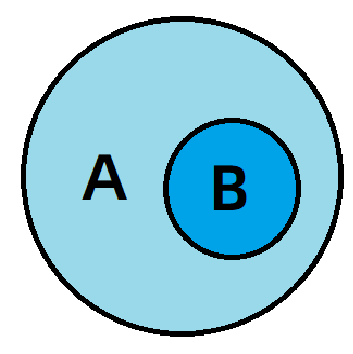
\includegraphics[width=0.1\textwidth]{image/Venn1.png}
  \caption{Venn图示例}
  \label{img:Venn1}
\end{figure}

\subsection{全集与补集}
  我们研究集合间的关系时,这些集合可能都是某一个给定的集合的子集,我们称这个给定的集合为\underline{全集}。我们一般记全集为$U$。比如说,解不等式时,我们默认全集为$\mathbb{R}$。

  接下来是补集。
\begin{definition}
  设全集为$U$,集合$A\subseteq U$,由$U$中所有不属于$A$的元素组成的集合称为$A$在$U$中的\underline{补集},记作${\complement}_{U}A$(若不会产生歧义,即只有一个全集的情况下,也可以记作$\overline{A}$或者$A^c$).读作“$A$在$U$中的补集”。即

  $${\complement}_{U}A=\{x|x\in I\text{,且}x\notin A\}.$$
\end{definition}
\begin{remark}
  此后如无特殊说明,我们默认$U$为全集。
\end{remark}
  然后来看几个例子。
\begin{example}
  $\complement_{U}A$用Venn图表示如图\ref{img:Venn3}所示,上色部分即为$\complement_{U}A$.
\end{example}
\begin{figure}[h]
  \centering
  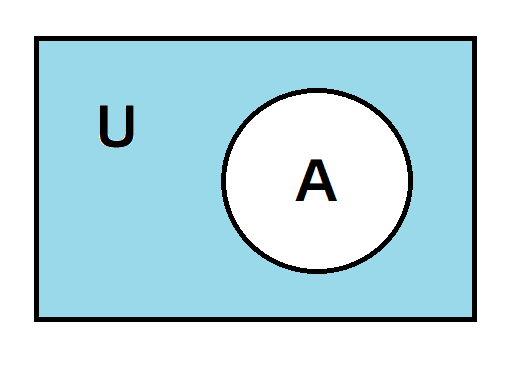
\includegraphics[width=0.2\textwidth]{image/Venn3.png}
  \caption{Venn图示例}
  \label{img:Venn3}
\end{figure}

\begin{example}
  设$U=\mathbb{R}$,则无理数集可以表示为$\overline{Q}$.
\end{example}

\begin{example}
  设$U=\mathbb{N}$,则$\overline{\mathbb{Z}^+}={0}$,这里的$\mathbb{Z}^+$表示正整数集。
\end{example}

下面是一个有趣的小例子。

\begin{example}
  设$A$为集合,则$\overline{\overline{A}}=A$.
\end{example}

\begin{example}
  设$U=\{1,2,3,4,5,6\}$,$A=\{2,3,4\}$,则$\complement_{U}A=\{1,5,6\}.$
\end{example}

\begin{example}
  设$U=\mathbb{R},A=\{x\mid -1<x<6\}$,则$\complement_{U}A=\{x\mid x\leq -1\text{或}x\geq 6\}.$
\end{example}

\subsection{交集与并集}
下面来看看集合的运算。
有时候,我们需要研究两个集合的公共部分。比如说,不等式中每个不等式解集的公共部分就是整个不等式组的解集。
\begin{definition}[交集]
  设$A$,$B$为两个集合,由$A$和$B$中的公共元素所组成的集合称为$A$和$B$的
  \underline{交集},记作$A\cap B$,即$$A\cap B=\{x\in A\text{ 且 }x\in B\}.$$
\end{definition}
  交集可以理解为两个集合相交的部分。
  用Venn图表示如图\ref{img:Venn2}。
  \begin{figure}[h]
    \centering
    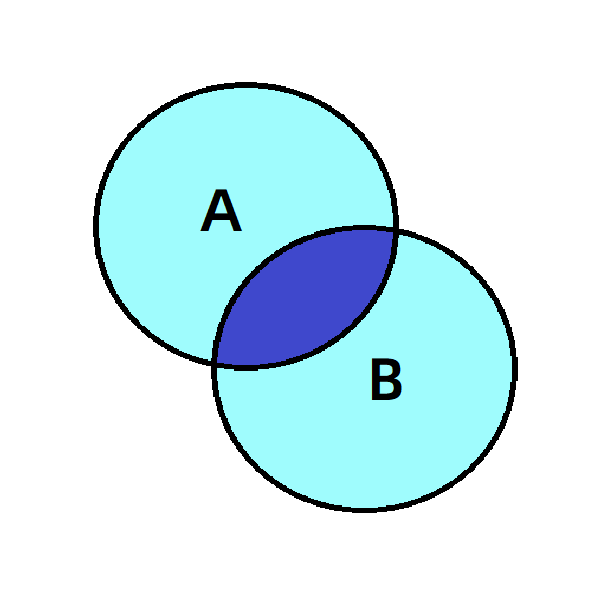
\includegraphics[width=0.2\textwidth]{image/Venn2.png}
    \caption{Venn图示例}
    \label{img:Venn2}
  \end{figure}
  图中深蓝色部分即为$A\cap B$。

\begin{definition}
  设$A$,$B$为两个集合,由$A$和$B$中所有元素组成的集合称为$A$和$B$的\underline{并集},记作$A\cup B$,即
  $$A\cup B=\{x\in A\text{或}x\in B\}$$
\end{definition}
  并集可以理解为两个集合合并且去掉重复元素后的部分。
  如图\ref{img:Venn2}所示,上色部分即为$A\cup B$。 

由这两个定义我们立刻可以得到这些常见的性质(更多的性质稍后介绍):

设$A$为集合,$U$为全集,则
\begin{property}
  零律:$A\cap\varnothing =\varnothing,A\cup\varnothing=A$;
\end{property}
\begin{property}
  同一律:$A\cap U=A;A\cup U=U$(这里$U$为全集).
\end{property}

\begin{exercise}\label{exer:10}
  用Venn图表示这两个定律。
\end{exercise}


这两个定律还是比较好理解的。所以我们直接快进到两个例子。

\begin{example}
  已知$A=\{1,2,3,4,5\},B=\{2,4,6\}$,则$A\cap B=\{2,4\}$,$A\cup B=\{1,2,3,4,5,6\}$.
\end{example}

\begin{example}
  若$A=\{\text{等腰三角形}\},B=\{\text{直角三角形}\}$,则$A\cap B=\{\text{等腰直角三角形}\}.$
\end{example}

\hspace*{\fill}

接下来需要提到的是条件的转换,或者说条件的翻译。来看这一个例子。
\begin{example}
  已知集合$A=\{x|x^{2}+4x=0\},B=\{x\|x^{2}+2(a+1)x+a^{2}-1=0\}.$

  (1)若$A\cap B=B$,求实数$a$的取值范围;(2)若$A\cup B=B$,求实数$a$的取值范围。
\end{example}
\begin{remark}
  这道题目的关键就是如何理解两个小题各自给出的条件:

  $A\cap B=B$说明$A$最起码也包含$B$中的所有元素,即$B\subseteq A$,同样地,$A\cup B=B$即$A\subseteq B$.

  还有,不要忘了\textcolor{red}{讨论空集},这是集合当中的火坑(每年都有一大批人被坑)。
\end{remark}
\begin{solution}
  $A=\{x\mid x^{2}+4x=0\}=\{-4,0\}.$
  (1)$\because A\cap B=B,$\enspace$\therefore B\subseteq A.$
  
  若$0\in B$,则$a^2-1=0,a=\pm 1.$当$a=1$时,$B=A$;当$a=-1$时,$B=\{0\}$,均满足条件。

  若$-4\in B$,则$a^2-8a+7=0,a=7\text{ 或 }1.$当$a=7$时,$B=\{-12,-4\}\nsubseteq A$,不满足条件。

  若$B=\varnothing$,则$\Delta=4(a+1)^{2}-4(a^{2}-1)<0$,解得$a<-1$.

  综上,实数$a$的取值范围为$(-\infty,-1]\cup\{1\}.$

  (2)$\because A\cup B=B,$\enspace$A\subseteq B.$

  $\because A=\{-4,0\},$\enspace$\therefore B$中至少有两个元素$-4,0.$

  $\because B$中的元素为一元二次方程的实根,

  $\therefore B$中至多有2个元素,

  $\therefore A=B.$

  由(1)可知此时$a=1$.
\end{solution}
\begin{remark}
  请注意一下(1)中取值范围的写法,每一段用并集符号连接,如果一段只有一个值,需要用花括号括起来。
\end{remark}

\hspace*{\fill}

集合的交与并运算具有一些性质,前三个与四则运算的性质是相似的,但是有一些不同。

设$A,B,C$均为集合,则
\begin{property}
  交换律:$A\cup B=B\cup A,A\cap B=B\cap A$;
\end{property}
\begin{property}
  结合律:$A\cup(B\cup C)=(A\cup B)\cup C,A\cap(B\cap C)=(A\cap B)\cap C$;
\end{property}
\begin{property}
  分配律:$A\cap(B\cup C)=(A\cap B)\cup(A\cap C),A\cup(B\cap C)=(A\cup B)\cap(A\cup C)$;
\end{property}

  结合律的集合运算符号是相同的,分配律的集合运算符号是不同的,请注意区别。

\begin{property}
  吸收律:$A\cup(A\cap B)=A,A\cap(A\cup B)=A.$
\end{property}

\begin{exercise}
  用Venn图表示这些定律。
\end{exercise}

\hspace*{\fill}

我们在这里证明其中三个。

\begin{example}
  证明上面集合运算的结合律。
\end{example}
\begin{proof}
  $(A\cap B)\cap C=\{x|x\in A\cap B\text{ 且 }x\in C\}=\{x|x\in A\text{ 且 }x\in B\text{ 且 }x\in C\}=\{x|x\in A\text{ 且 }x\in B\cap C\}\\=A\cap(B\cap C).\\(A\cap B)\cap C=\{x|x\in A\cup B\text{ 或 }x\in C\}=\{x|x\in A\text{ 或 }x\in B\text{ 或 }x\in C\}=\{x|x\in A\text{ 或 }x\in B\cup C\}\\=A\cup(B\cup C).$

  Q.E.D.
\end{proof}
\begin{remark}
  Q.E.D.表示证明完毕,是拉丁文"quod erat demonstrandum"的缩写。
\end{remark}

\hspace*{\fill}

\begin{example}
  证明上面集合运算的分配律。
\end{example}

  和例\ref{exap:2}类似,我们用定义来证。但是这里只证明前一个,另外一个留作练习。

\begin{proof}
  首先证明$A\cap(B\cup C)\subseteq(A\cap B)\cup(A\cap C)$.

  \textcolor{cyan}{任取}\enspace$x\in A\cap(B\cup C)$,那么$x\in A\text{ 且 }x\in B\cup C$.

  若$x\in B$,由于$x\in A$,那么$x\in A\cap B$;

  若$x\in C$,由于$x\in A$,那么$x\in A\cap C$.

  所以$A\cap(B\cup C)\subseteq(A\cap B)\cup(A\cap C)$.

  \hspace*{\fill}

  再证明$(A\cap B)\cup(A\cap C)\subseteq A\cap(B\cup C)$.

  \textcolor{cyan}{任取}\enspace$x\in (A\cap B)\cup(A\cap C)$,那么$x\in A\cap B\text{ 或 }x\in A\cap C$.

  若$x\in A\cap B$,则$x\in B\cup C\text{且}x\in A$,所以$x\in a\cap(B\cup C)$;

  若$x\in A\cap C$,则$x\in B\cup C\text{且}x\in A$,所以$x\in a\cap(B\cup C)$.

  所以$(A\cap B)\cup(A\cap C)\subseteq A\cap(B\cup C)$.

  综上,$A\cap(B\cup C)=(A\cap B)\cup(A\cap C).$

  Q.E.D.
\end{proof}
\begin{remark}
  请特别注意,我们需要“任取”,这样才比较严谨。
\end{remark}

\hspace*{\fill}

\begin{example}
  证明上面集合运算的吸收律。
\end{example}
关于这个定律的证明,我们使用的是引入其它集合(全集和空集)。

\begin{proof}
  $A\cup (A\cap B)=(A\cap U)\cup(A\cap B)=A\cap(B\cup U)=A\cap U=A.$

  (第二步逆用了分配律,最后两步用到了同一律。)

  $A\cap(A\cup B)=(A\cup\varnothing)\cap(A\cup B)=A\cup(B\cap\varnothing)=A.$

  (第二步逆用了分配律,最后一步用到了零律。)
\end{proof}

\subsection{习题}

\begin{exercise}\label{exer:11}
  集合$\{0\}$与$\varnothing$是否相等?它们满足什么关系?
\end{exercise}
\begin{exercise}\label{exer:12}
  证明:$\text{如果}A\subseteq B,B\subseteq S,\text{那么}A\subseteq S$.
\end{exercise}
\begin{exercise}\label{exer:13}
  $\text{已知集合}A=\{1\text{,3,}m\}\text{,}B=\{m^2\text{,1}\}\text{,且}A\cup B=A\text{,求}m\text{的值}.$
\end{exercise}
\begin{exercise}
  $\text{设}U=\{x\mid x{\in}N,\text{且}x{\leqslant}10\},A=\{1,2,4,5,9\},B{=}\{4,6,7,8,10\},C=\{3,5,7\},\text{求}A\cap B,A\cup B,\bar{A}\cap\bar{B},\bar{A}\cup\bar{B},(A\cap B)\cap C,(A\cup B)\cup C.$
\end{exercise}
\begin{exercise}\label{exer:14}
  $\text{已知}A=[-1,2],B=\left(-\infty,-\frac{p}{4}\right),\text{且}B\subsetneqq{\complement}_{\mathbb{R}}A\text{,求实数}p\text{的取值范围}.$
\end{exercise}
\begin{exercise}
  我们记集合$A$的元素个数为$\mid A\mid$.

  (1)用Venn图说明:$|A\cup B|=|A|+|B|-|A\cap B|$.

  (2)用Venn图说明:$|A\cup B\cup C|=|A|+|B|+|C|-|A\cap B|-|B\cap C|-|C\cap A|+|A\cap B\cap C|$.

  这其实是集合的容斥原理。
\end{exercise}
\begin{exercise}
  $\text{设}x,y,z\text{都是非零实数,试用列举法将}\frac x{|x|}+\frac y{|y|}+{\frac{z}{\mid z\mid}}+{\frac{xy}{\mid xy\mid}}+{\frac{xyz}{\mid xyz\mid}}\text{的所有可能值构成的集合表示出来}.$
\end{exercise}
\begin{exercise}
  设 A 是两个整数平方和的集合,即$A=\{x\mid x=m^2+n^2,\:m,\:n\in\mathbb{Z}\}.$

(1)证明:若 $s,t{\in}A$,则 $st{\in}A$;

(2)证明:若 s, $t\in A,t\neq0$,则$\frac st=p^2+q^2$,其中 $p,q$ 是有理数.
\end{exercise}
\end{document}
